\documentclass{tufte-handout}
\usepackage{graphicx}
\usepackage{multicol}
\usepackage{hyperref}
\usepackage{mdwlist}
% Set font to Charter
\usepackage[bitstream-charter]{mathdesign}
\usepackage[T1]{fontenc}
% Filter out unwanted warnings and error messages
\usepackage{silence}
  \WarningFilter{latex}{Marginpar}
  
\title{Wiisel: Project Report}
\author{Team: Hala Diab, Sam Friedman, Joe Wright}
\date{19 December - EE C149 Fall 2014}

\begin{document}
\maketitle
\begin{abstract}
    A user will be able to use a Nintendo Wiimote to draw on a large screen of
LEDs changing colors depending
on drawing ``mode'' and sensor input. Drawing modes include monotone, color selected by user among a set of colors.User will also be able to switch to display mode for a slide show of bitmap images.
\end{abstract}

\section{\textbf{System Structure}}

\begin{marginfigure}
    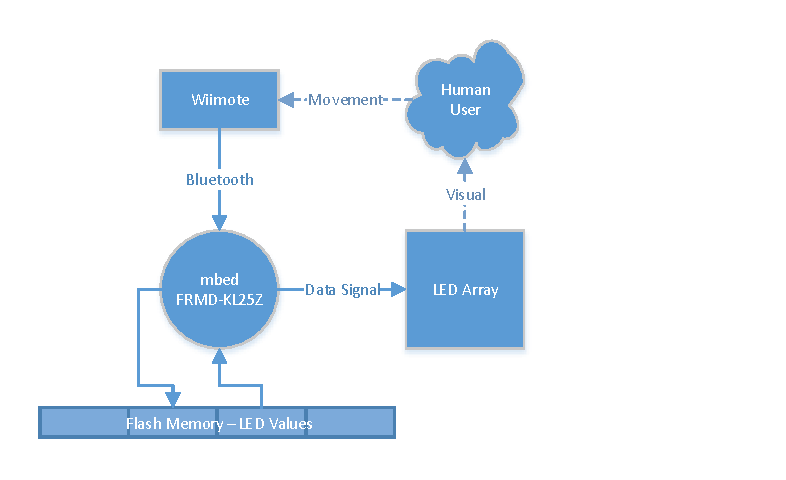
\includegraphics[trim=1cm 0cm 4cm 0cm, width=\linewidth]{dataflow.pdf}
    \caption{Data Flow and Project Structure}
\end{marginfigure}
\begin{marginfigure}
    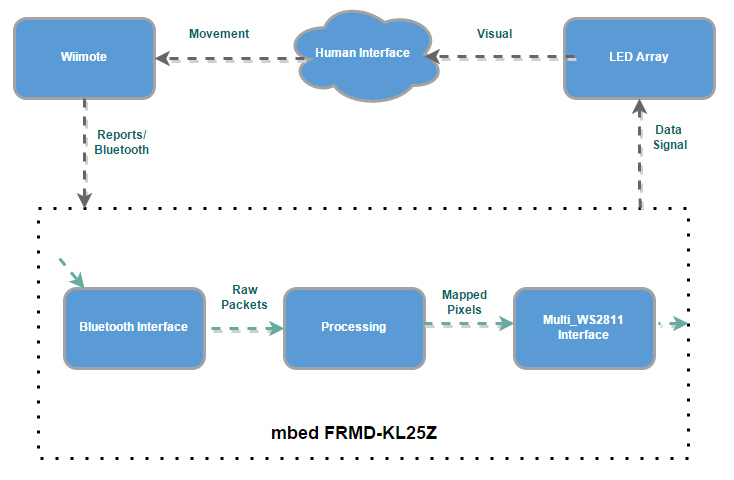
\includegraphics[trim=3cm 0cm 4cm 0cm, width=\linewidth]{dataflow1.png}
    \caption{Detailed Data Flow}
\end{marginfigure}
Figure 1 shows an abstract view of the system components and how they interact with each other.\\Figure 2 shows more details about the interaction between Wiimote, Screen, and the microprocessor.
\section{\textbf{System Components}}
\underline{\textit{\textbf{Need to Explain Selection of Components}}}
\subsection{Screen of Neopixels:}
The screen is 1 meter by 1 meter, with a 30x30 resolution, and
is made of WS2812b individually addressable LEDs. It consists of: 15 strips with 30 LEDs/strip and 15 strips with 60 LEDs/strip.
\subsection{Freescale mbed FRMD-KL25Z}:
A 32-bit ARM Cortex microcontroller that runs at 48MHz, has 128kB of Flash storage for code, 16kB of RAM for variables.
\subsection{Wiimote:}
The Nintendo Wiimote is the sensor platform.This includes a 3-axis accelerometer and several buttons. The Wiimote interfaces with the microcontroller over bluetooth using a Bluetooth CSR 4.0 USB dongle that is connected to the microcontroller using USB OTG.
\section{\textbf{Building the System}}
\underline{\textbf{\textit{Add the wiring diagram of data pins to mbed + add figure to show power every 4 strips }}}
\begin{figure}
    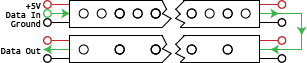
\includegraphics{Wiring_Diagram.png}
    \caption{LED Strip Wiring. A 1 meter length of 30 LED per meter strip is
    attached to the end of a 1 meter length of 60 LED per meter strip. This
lets us connect fifteen total strips of 90 LEDs to the microcontroller,
instead of thirty strips. The software needs to have some model of the
physical arrangement of LEDs, so that it can properly address each LED.}
\end{figure}
\section{\textbf{Software}}
\subsection{Screen Control}
To control the LEDs, we are using the Multi\_WS2811 library\sidenote{This
library is by Ned Konz for the FRDM-KL25Z, and is made available to us under
the Apache License.} This library can control up to 16 strips of LEDs in
parallel using 3-phase DMA transfers\sidenote{The number of parallel LED
strips is limited to at most the number of pins on a single GPIO port for the
microcontroller.}. 
\subsection{Wiimote}
Data Packets from Wiimote are reported over Bluetooth to mbed where it processes the packets using a bluetooth stack built on top of usb software interface:
\begin{enumerate*}
    \item
        \textbf{KL46Z-USBHost}\sidenote{\url{http://developer.mbed.org/users/va009039/code/KL46Z-USBHost/}}:
a simple USBHost library for FRDM-KL46Z(FRDM-KL25Z) by Norimasa Okamoto, under MIT and Apache license.
\item
    \textbf{KL46Z-BTstack}\sidenote{\url{http://developer.mbed.org/users/va009039/code/KL46Z-BTstack_example/}}:
a Bluetooth Stack (built on top of KL46Z-USBHost) by Norimasa Okamoto. Supports L2CAP protocol used by the Wiimote.
\end{enumerate*}
We processed packets to extract acceleration and buttons values. To get accurate acceleration values, we had to calibrate the wiimote we used. Assuming that bias and sensitivity are roughly equal along all axes, we modeled wiimote as an affine model\sidenote{Affine Model : f(x) = ax+b}: $f(x) = 102x + 486 $. Then roll and pitch were calculated using following equations\sidenote{Source:Implementing a Tilt-Compensated eCompass using Accelerometer and Magnetometer Sensors by Talat Ozyagcilar}:\\
$ roll = arctan(\frac{x}{z}) , pitch = arctan(\frac{y}{x sin(roll) + z cos(roll)})$
\section{\textbf{Testing and Verification}} 
We started testing in early phases in the project. We started by testing screen control software on individual LED strips to confirm that data signals are sent correctly from microcontroller to strips. This and the difference between power connection and the daisy chaining of data wires made it easier to test hardware issues.\\
\underline{\textbf{\textit{Add screenshots from oscilloscope when testing the noise }}}
\section{\textbf{Analysis}}
\subsection{Power}
Although datasheets for the specific model of LED strips we have were not
available, a common upper-bound\sidenote{This occurs when the LED is set to
full brightness white. Average consumption is much lower} for WS2812b-based 
LEDs is 60 mA per LED\sidenote{Burgess, Phillip.``Powering NeoPixels.''
    \textit{Adafruit}. 30 Aug 2013. Web.
    \url{https://learn.adafruit.com/adafruit-
    neopixel-uberguide/power}}. Average-case current draw is typically around
    20 mA. For an array of 900 LEDs, this comes out to a total current draw
    from 18 A to 54 A at 5 volts. To make the system as safe as possible, we designed the
    LED array hardware to distribute this current evenly and
    handle peak usage without catching fire. We also drastically lowered the ``Peak usage'' by limiting the LED brightness in software, and designing the
    system behavior to reduce the frequency of high current draw
    states.\sidenote{The default ``blank'' screen is non-white. If the LEDs are off
        instead of white, then initially the array will use very little power,
    instead of the maximum possible.}
    We Measured power values and found that we consume 93 W when screen is Red with full brightness. Changing mode to 15\% brightness, power consumption is decreased to 37 W.
\subsection{Latency}

\subsection{Memory Usage:}
As initially written, Multi\_WS2811 library cannot support the number of LEDs per strip that we need it to in the available amount of RAM on the device. At 80 LEDs per strip, the library takes approximately 98\% of the RAM on the microcontroller. To remedy this, we moved a large run-time constant array from RAM to Flash\sidenote{The downside to this approach is that we must now hardcode all values of the array instead of using \texttt{memset}, which requires more work on the part of the programmer, but does not affect functionality of the library.}, which reduced RAM usage to 57\% at 90 LEDs per strip. We also compressed the color representation from 24 bits/pixel to 12 bits/pixel.

\section{Future Work}
We plan to add more sensors to make pointing and drawing easier like adding IR sensors. We also plan to add more features like changing brush size, displaying text, and saving drawn pictures to SD card.

\end{document}
